
\begin{figure}
    \centering
    \subfloat[]{
        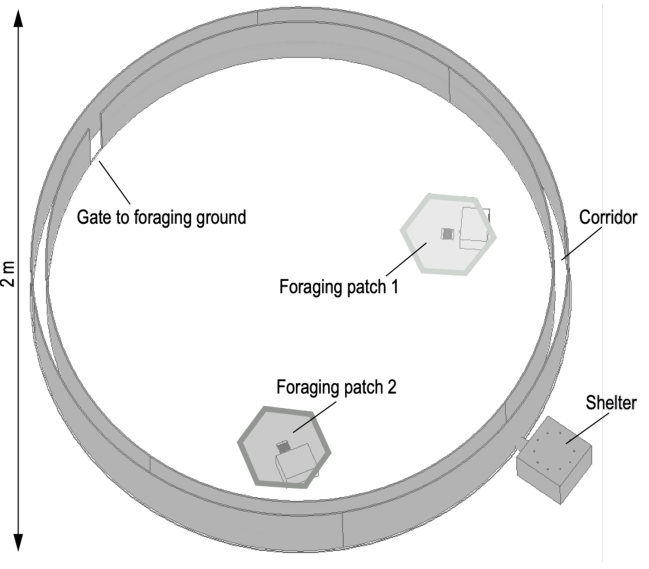
\includegraphics[width=4in]{figures/arena.png}
    }
    \hfill
    \subfloat[]{
        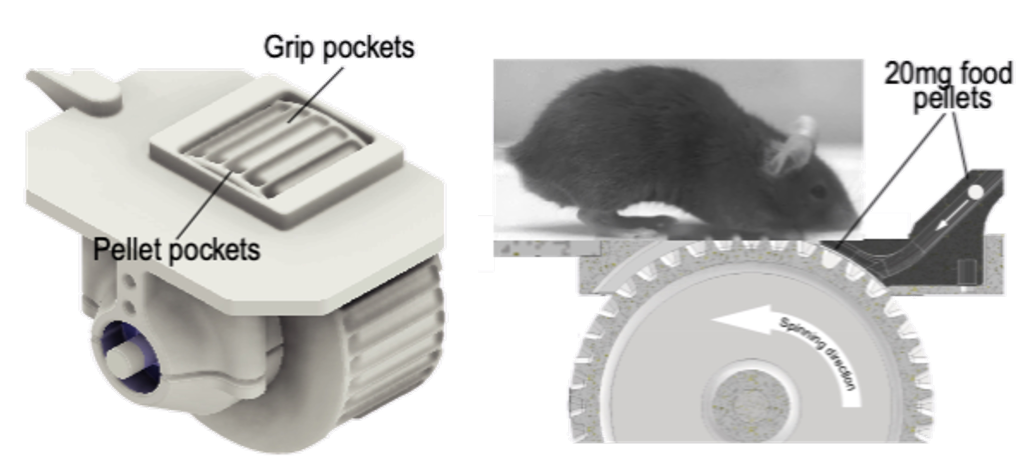
\includegraphics[width=4in]{figures/patch.png}
    }
    %
    \caption{Foraging arena (a) and feeder (b).
    %
    The floors of the arenas are tessellated to form honeycombs of modular
    hexagonal tiles (a), each of which can be equipped with a newly designed
    underground feeder (b).
    %
    Pellets are dispensed onto a foraging wheel once the mouse has spun it for
    a pre-defined programmable distance threshold using its forepaws (fictive
    digging).
    %
    The arena contains up to six scale-equipped nesting modules that allows
    housing of mice in the arena and weight monitoring.
    %
    Behavioural monitoring is achieved by an array of high-speed cameras (up to
    15), by which mouse location, mouse identity and body parts can be track in
    real time.
    %
    Long term monitoring of neural activity is performed using Neuropixels
    probes.
    %
    }
    %
    \label{fig:arena}
\end{figure}
